\documentclass[conference]{IEEEtran}
\IEEEoverridecommandlockouts
% The preceding line is only needed to identify funding in the first footnote. If that is unneeded, please comment it out.
\usepackage{cite}
\usepackage{amsmath,amssymb,amsfonts}
\usepackage{algorithmic}
\usepackage{graphicx}
\usepackage{textcomp}
\usepackage{xcolor}
\def\BibTeX{{\rm B\kern-.05em{\sc i\kern-.025em b}\kern-.08em
    T\kern-.1667em\lower.7ex\hbox{E}\kern-.125emX}}
\begin{document}

\title{Interaktive Pflanzenüberwachung im Smart Home ohne dedizierte Access Points \\

}

\author{\IEEEauthorblockN{Michael Jathe}
\IEEEauthorblockA{\textit{Department 2} \\
\textit{Hochschule Hamm-Lippstadt}\\
Lippstadt, Deutschland \\
michael.jathe@stud.hshl.de}
}

\maketitle



\begin{IEEEkeywords}
smart home, mqtt, plants, automation
\end{IEEEkeywords}
\section{Motivation}
Der Smart Home Sektor befindet sich seit Jahren in einem stetigen Wachstum. Die Zahl der Hersteller von Smart Home Produkten nimmt zu und die Automatisierung und Überwachung breitet sich auf alle Bereiche im Haus aus. Aktuell ist die Entwicklung von Geräten zur Pflanzenüberwachung bei vielen Herstellern im Fokus. 


Wichtige Aspekte des Smart Homes sind die Kommunikation zwischen den Sensoren/Aktoren, die Anbindung an das Internet und die Steuerung per Smartphone. Ein verbreiteter Standard dafür ist der KNX Feldbus. Aufgrund des hohen Installationsaufwand und den hohen Kosten wird dieser allerdings meist nur im professionellen Bereich eingesetzt. Zudem ist er nicht einfach nachrüstbar, sodass er nur in Neubauten oder kernsanierten Gebäuden zum Einsatz kommt.


Daher haben die meisten Hersteller ihre eigenen System entwickelt. Für die Anbindung der Sensoren und Aktoren wird ein eigener Access Point benötigt. Der Datenaustausch findet über Funk, WLAN oder Ethernet statt über ein Herstellereigenes Protokoll statt. Für die Internetanbindung wird meist eine eigene Cloudlösung angeboten oder der Access Point wird über Portfreigaben von aussen ereichbar gemacht, was ein erhebliches Sicherheitsrisiko mit sich bringt. Ein Vorteil dieser Systeme ist die einfache und kostengünstige Nachrüstung. 
\begin{figure}[h]
    \centering
    \includegraphics[width=1\linewidth]{top.jpg}
    \caption{Mehrere Access Points im Smart Home }
    \label{fig:top}
\end{figure}

Da sich die Hersteller nicht auf einen gemeinsamen Standard geeinigt haben, sind die Systeme von verschiedenen Herstellern meist nicht miteinander kompatibel. Daher müssen sich die Nutzer entweder auf das Produktangebot eines Herstellers beschränken oder für jeden weitern Hersteller einen zusätzlichen Access Point installieren. Zudem wird jedes System eine eigene App zur Interaktion benötigt.

Ziel dieser Arbeit ist es, ein System aus Sensoren und Aktoren zur Pflanzenüberwachung zu entwickeln, welches ohne einen dedizierten Access Point auskommt und unter bestimmten Vorraussetzungen in bestehende Systeme eingebunden werden kann.
\section{Anforderungen}
\begin{itemize}
    \item Das System muss ohne dedizierten Acces Point auskommen.
    \item Jeder Knoten muss auch als Access Point/Broker fungieren können.
    \item Bei Ausfall des Access Points/Brokers wird muss das System selbständig einen neuen Broker bestimmen.
    \item Bei Ausfall des Brokers darf kein Datenverlust entstehen.
    \item Der Broker muss die gesammelten Daten in eine Cloud übertragen
    \item Die Daten müssen über eine Weboberfläche oder App abrufbar sein.

\end{itemize}
\section{Konzept}
Es soll ein System entwickelt werden, in dem jeder Knoten, das heißt Sensor, Aktor oder Bedienelement, auch die Funktion des Access Point übernehmen kann. Für die Kommunikation wird MQTT(Message Queuing Telemetry Transport) eingesetzt. MQTT ist ein offenes Netzwerkprotokoll für Machine-to-Machine-Kommunikation (M2M), das die Übertragung von Telemetriedaten in Form von Nachrichten zwischen Geräten ermöglicht.
MQTT beruht auf dem Client-Server-Modell. Der Server, auch Broker genannt, stellt den Clients Kanäle zur Kommunikation zur Verfügung. Die Clients können diese Kanäle anlegen, auf Ihnen Nachrichten veröffentlichen und sie abonnieren, um Nachrichten von anderen Clients zu empfangen. 

Bei der Konfiguration des ersten Knoten/Clients wird dieser als Broker festgelegt. Alle weiteren Clients melden sich bei dem Broker an. Der Broker speichert legt eine Tabelle mit allen Clients und deren IP-Adressen an. Sobald sich ein neuer Client anmeldet, wird die aktualisierte IP-Tabelle an alle Clients gesendet. Das geschieht über einen MQTT-Kanal dem alle Clients folgen.

\begin{figure}[h]
    \centering
    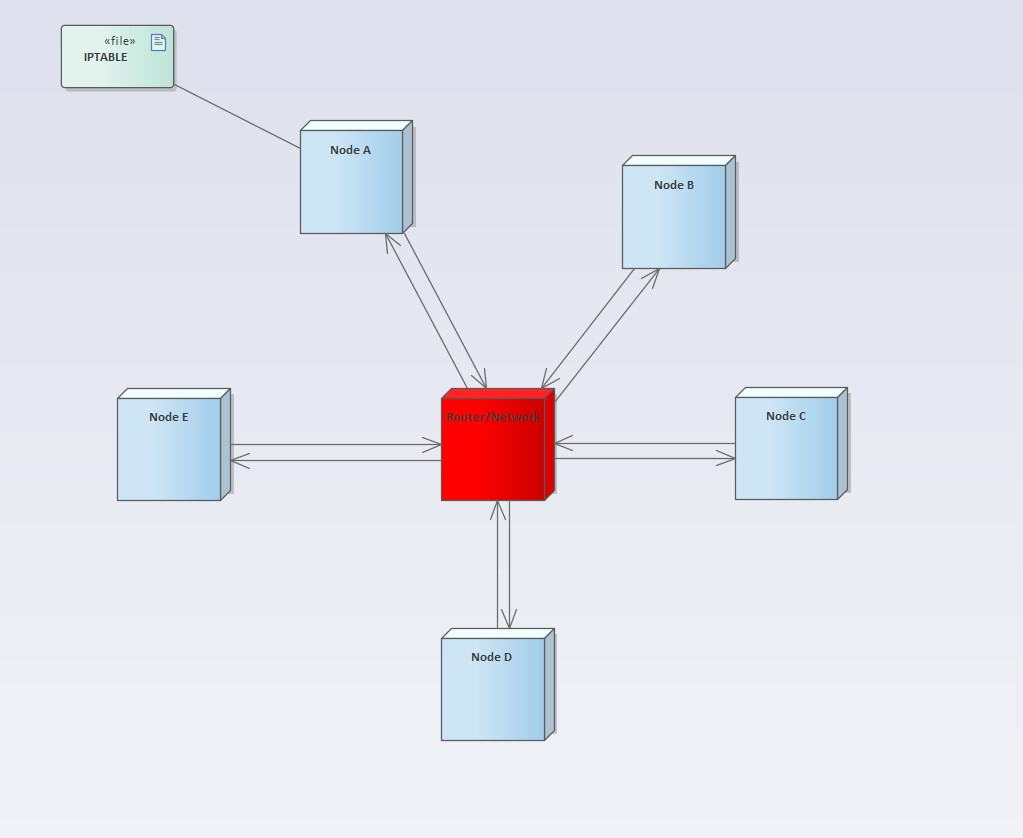
\includegraphics[width=1\linewidth]{network_scratch.jpg}
    \caption{MQTT Netzwerk/ Jeder Knoten kann Broker werden}
    \label{fig:statemachine}
\end{figure}

Der zweite Client, der sich beim Broker anmeldet wird in der IP-Tabelle als Backup-Broker angelegt. Sollte der Broker abstürzen, übernimmt der Backup-Broker die Rolle des Brokers und bestimmt einen neuen Backup-Broker. Sobald der abgestürzte Broker wieder betriebsbereit ist, meldet er dies dem neuen Broker und übernimmt wieder seine alte Position. Sollte durch den Absturz die IP-Tabelle verloren gegangen sein, muss das Gerät neu konfiguriert werden.

Der Broker hat außerdem die Aufgabe, alle Daten der Clients zu sammeln und diese kurzen Abständen in einer Cloud zu hinterlegen. 
\begin{figure}[h]
    \centering
    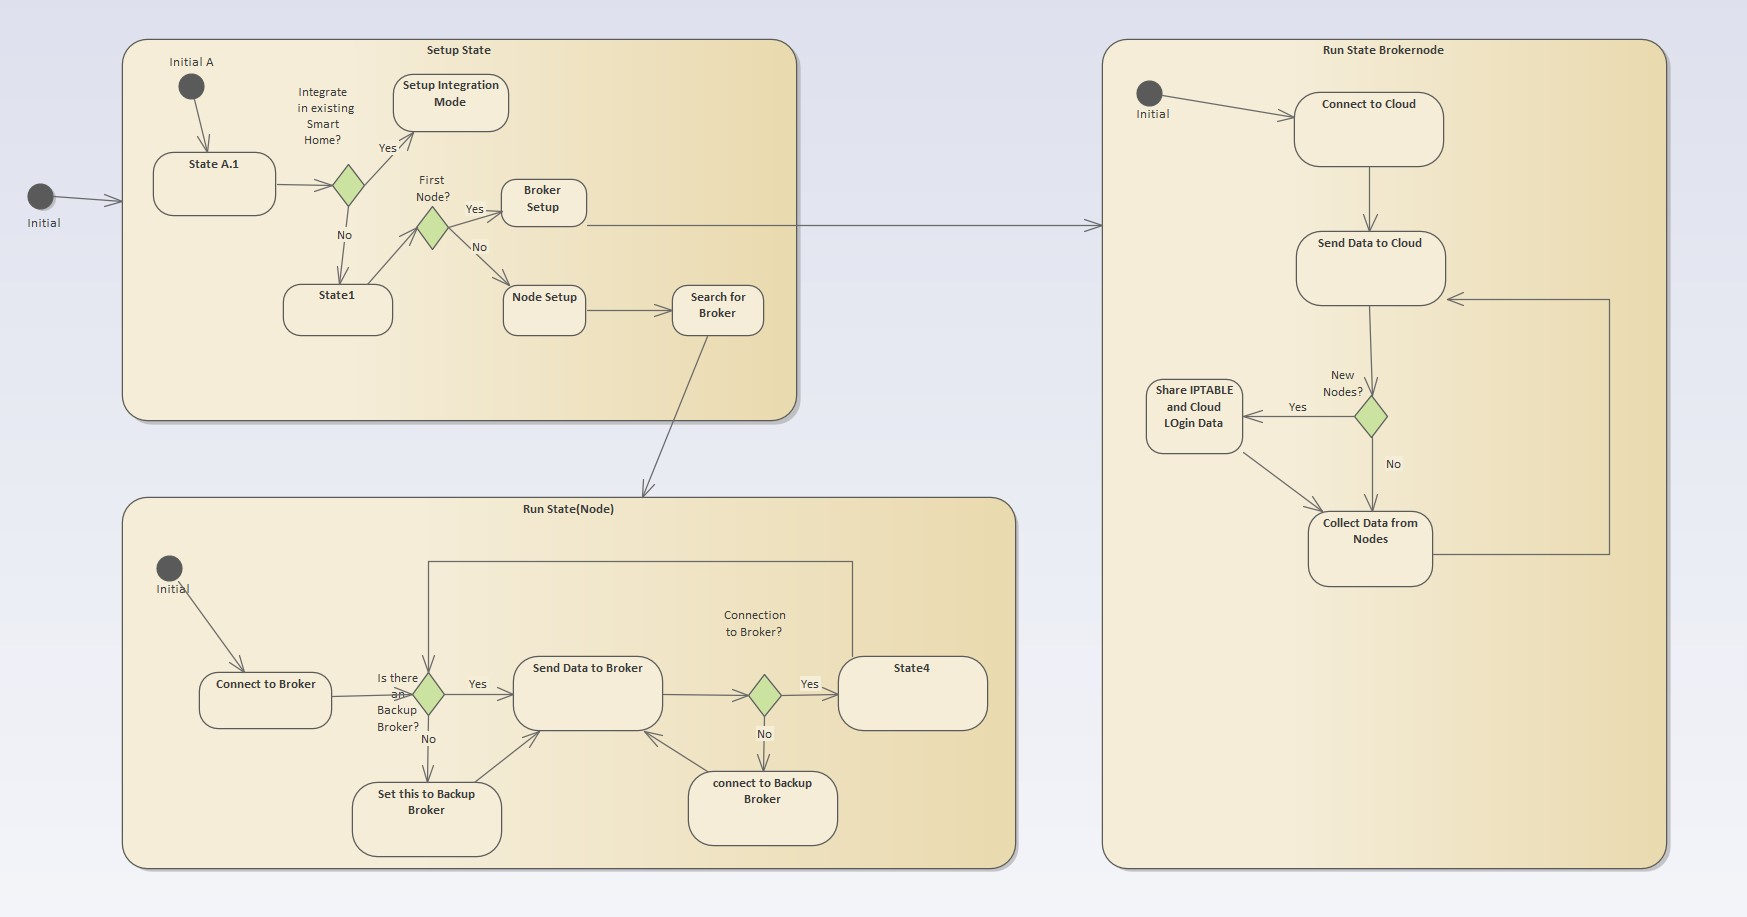
\includegraphics[width=2\linewidth]{state_machine.jpg}
    \caption{Konfiguration als Node oder Broker/Node}
    \label{fig:statemachine}
\end{figure}
\begin{thebibliography}{00}
%\bibitem{b1} G. Eason, B. Noble, and I. N. Sneddon, ``On certain integrals of Lipschitz-Hankel type involving products of Bessel functions,'' Phil. Trans. Roy. Soc. London, vol. A247, pp. 529--551, April 1955.
%\bibitem{b2} J. Clerk Maxwell, A Treatise on Electricity and Magnetism, 3rd ed., vol. 2. Oxford: Clarendon, 1892, pp.68--73.
%\bibitem{b3} I. S. Jacobs and C. P. Bean, ``Fine particles, thin films and exchange anisotropy,'' in Magnetism, vol. III, G. T. Rado and H. Suhl, Eds. New York: Academic, 1963, pp. 271--350.
%\bibitem{b4} K. Elissa, ``Title of paper if known,'' unpublished.
%\bibitem{b5} R. Nicole, ``Title of paper with only first word capitalized,'' J. Name Stand. Abbrev., in press.
%\bibitem{b6} Y. Yorozu, M. Hirano, K. Oka, and Y. Tagawa, ``Electron spectroscopy studies on magneto-optical media and plastic substrate interface,'' IEEE Transl. J. Magn. Japan, vol. 2, pp. 740--741, August 1987 [Digests 9th Annual Conf. Magnetics Japan, p. 301, 1982].
%\bibitem{b7} M. Young, The Technical Writer's Handbook. Mill Valley, CA: University Science, 1989.
\end{thebibliography}



\end{document}
